\section{Results}

\subsection{Unoptimized Beam}

The experiment to determine the contact potential of the sample-gun system can be performed using any configuration for the gun and in a very short 
amount of time. The utility of the contact potential made this the most logical first step. By setting $V_g$ to 15V and biasing the sample 
from 0V to 20V, we obtain the results shown in Figure \ref{fig:contact}. This measurement was repeated a total of three times. 
The value $V_s$ is determined by finding the first bias voltage at which the sample current begins to increase, and it was found to be 
$8.37\pm0.05$V. Recalling equation \eqref{vgvs} we find that the contact potential for this specific system is $\Delta = 6.63\pm0.05$eV.

\begin{figure}[h!]
	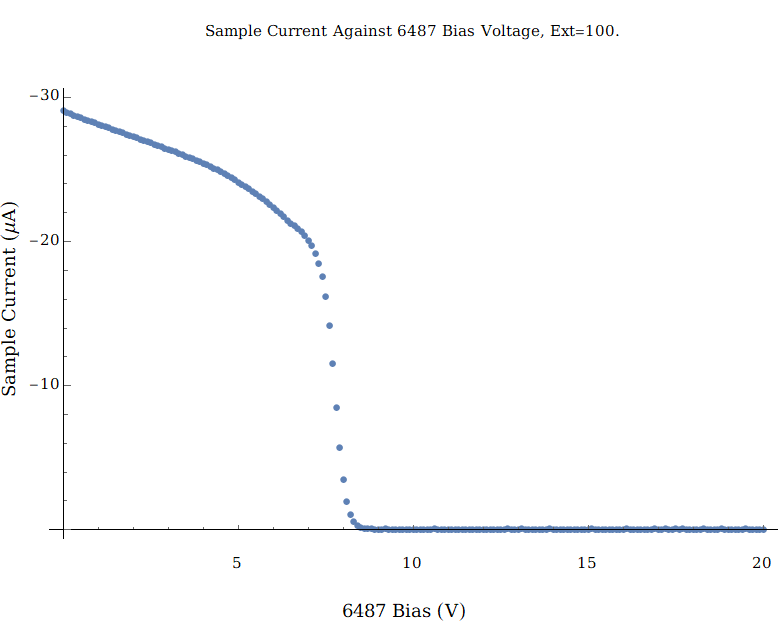
\includegraphics[width=0.32\linewidth]{../Test Scans/GunResPlots/Plot1_Ext100.GunResTest.png}
	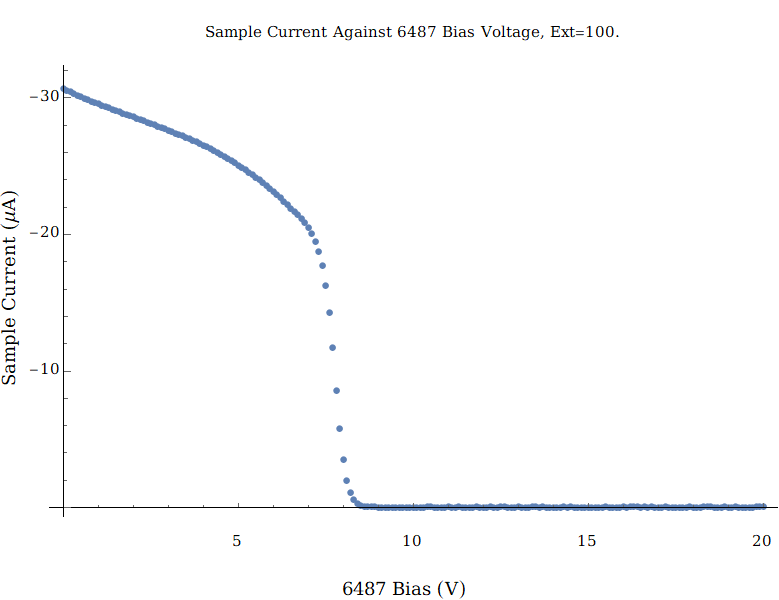
\includegraphics[width=0.32\linewidth]{../Test Scans/GunResPlots/Plot2_Ext100.GunResTest.png}
	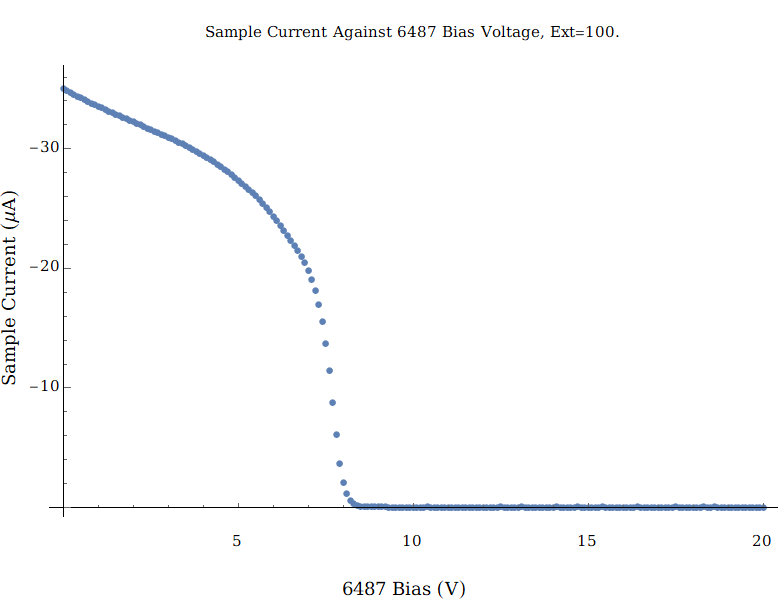
\includegraphics[width=0.32\linewidth]{../Test Scans/GunResPlots/Plot3_Ext100.GunResTest.png}
	\caption{Sample current against sample bias voltage for contact potential determination}
	\label{fig:contact}
\end{figure}

Unlike determining the contact potential, the process of finding optimal values from a parameter space this large is a challenging task. Thankfully the manufacturer of the electron gun used provided a list of starting parameters
which were recommended for an electron energy of 15eV. With the values in table \ref{tab:recpar} applied to our gun, we started by measuring its width along both the $x$ and 
$z$ directions. The beam was found to be roughly 15mm wide in both directions, an order of magnitude too large for use in IPES. Further we see that the beam appears to be more 
concentrated towards its edge, meaning that at this configuration the beam is poorly collimated in addition to being too large. 

\begin{table}[h!]
	\centering
	\begin{tabular}{ccccccc}
		\hline
		\multicolumn{1}{l|}{Paremeter} & Filament* & Energy & Extraction* & Grid & Focus 1 & Focus 2 \\ \hline
		\multicolumn{1}{l|}{Value (V)} & 5.0 & 15.0 & 100.0$\rightarrow$50.0 & -13.4 & 8.0 & -9.3 \\ \hline
	\end{tabular}
	\caption{Starting parameters recommended by Staib Instruments for the NEK-150 low energy electron gun at $E_i=15$eV. A recommended filament 
	voltage was not provided, so it was chosen arbitrary. Finally, using the recommended extraction value of 100V was not possible since it caused 
	the emission current of the gun to exceed its safe maximum value. To protect the filament we had to turn the extraction down to 50V.}
	\label{tab:recpar}
\end{table}

\begin{figure}[h!]
    \centering
    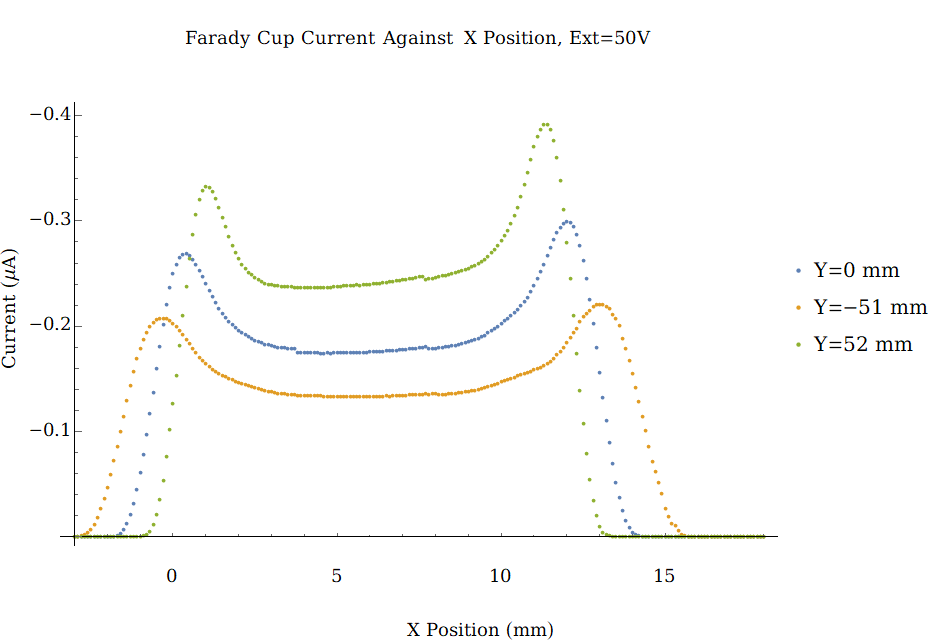
\includegraphics[width=0.45\linewidth]{../Test Scans/GunResPlots/BeamWidthXVaryingYExt50.png}
	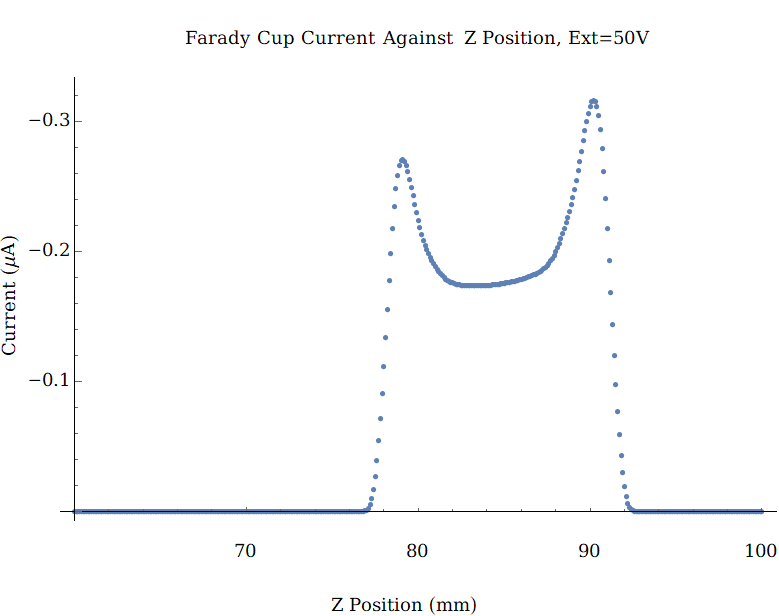
\includegraphics[width=0.45\linewidth]{../Test Scans/GunResPlots/BeamWidthZExt50.png}
	\caption{Beam width measurements taken using recommended operating parameters. Left: Beam current against $x$ position at different working distances. Increasing $y$ position is closer to output of electron gun. 
	Right: Beam current against $z$ position, at fixed working distance}
    \label{fig:badbeam}
\end{figure}

In order to corroborate these observations of an unexpected beam shape, we focused the Farady cup at three specific regions of interest within the beam.
At the left peak ($x=1$mm), the beam centre ($x=6$mm), and the right peak ($x=13$mm) we biased the cup with a potential ranging from 0V to 20V to probe the 
beam's energy spread. The results in figure \ref{fig:enres} show that the electrons at the beam's edge are easily repelled by small voltage 
biases. Comparing this to the electrons at the centre of the beam and we find that the current remains constant for increasing bias until reaching the 
threshold value where it quickly drops to zero. So while the beam has a higher concentration of electrons towards its edge, the energy distribution 
is more broad than at the beam's centre and thus contains a higher proportion of low energy electrons. 

\begin{figure}[h!]
    \centering
    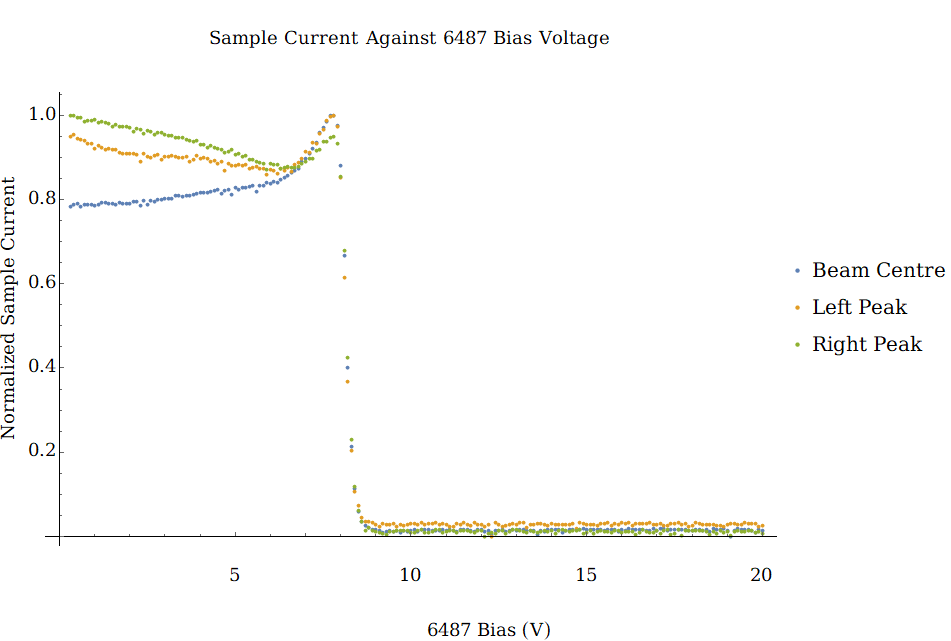
\includegraphics[width=0.85\linewidth]{../Test Scans/GunResPlots/ContactPotentialLocationsInBeam.png}
	\caption{Current of electron beam against Faraday cup bias voltage, for beam set to recommended operating conditions. The three locations correspond to 
	the features shown in figure \ref{fig:badbeam} and are at $x$ positions of 6mm, 1mm, and 13mm in order of appearance in plot legend.}
    \label{fig:enres}
\end{figure}

After obtaining these results we shifted focus to prioritize obtaining a gaussian beam profile above every other requirement. Referring back to 
table \ref{tab:recpar} we see that the filament voltage was the only free parameter we had when using the manufacturer recommended values. For simplicity
we chose the maximum value of 5V, which means the cathode is operating at its highest temperature. We hypothesized that at this high temperature, 
the broadened thermal energy distribution of electrons emitted from the cathode could lead to the broadening of the beam's shape and an excess of 
low energy electrons towards the beams edges. This hypothesis was tested by decreasing the filament voltage to lower the cathode's temperature.

\subsection{Lowered Temperature}

Our first test used a filament voltage of 4.5V, which allowed us to increase the extraction to the recommended 100V. 
Figure \ref{fig:firstgauss} shows that in this new configuration we do manage to obtain a gaussian profile, 
though its FWHM is roughly 8mm which is far too large for IPES. The discontinuities in the plot were caused by a loose backlash screw in the 
motor assembly, which was later fixed.

\begin{figure}[h!]
    \centering
    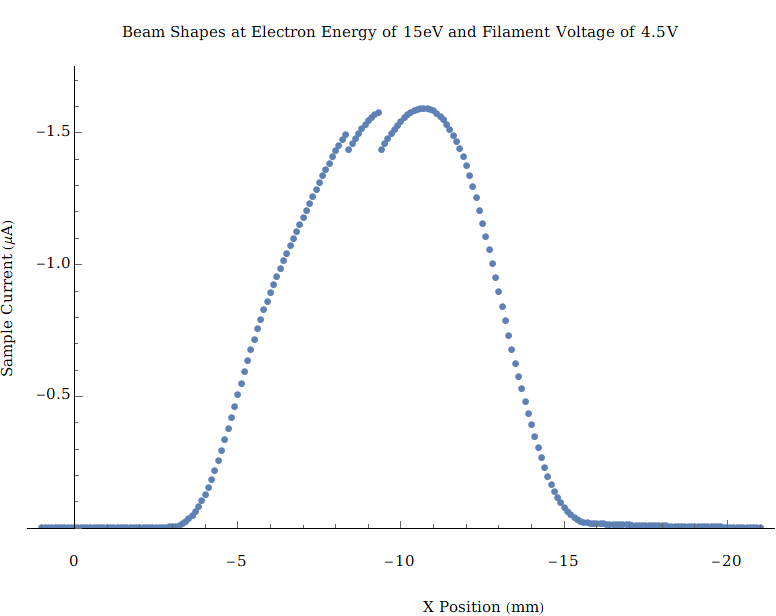
\includegraphics[width=0.85\linewidth]{../Work Term Replication/Plots/Work Term Replication E15Fil4.5.png}
	\caption{Beam current against Faraday cup $x$ position for reduced filament voltage of 4.5V, all other parameters remained unchanged from 
	table \ref{tab:recpar}.}
    \label{fig:firstgauss}
\end{figure}

While it is true we were able to increase the extraction to 100V, this configuration was not stable and the emission current slowly grew until it 
reached the maximum safe value of 100$\mu$A. Decreasing the filament voltage to 4V allowed for the beam to be operated at 100V extraction indefinitely. This was 
the filament voltage we decided to use for the remainder of the optimization. To make quicker work of this optimization problem we chose to alter the 
remaining values in large steps, exploring a wide range of parameter space. Similarly designed electron guns report achieving good performance when
the focus potential is roughly comparable to the extraction potential\cite{stoffel1985low,raj2004optimization}. This allowed us to limit our search even further by placing more emphasis 
on beam configurations where $F_1$ or $F_2$ were 100V. Figure \ref{fig:workterm} shows the beam widths at eight different configurations.

\begin{figure}[h!]
    \centering
    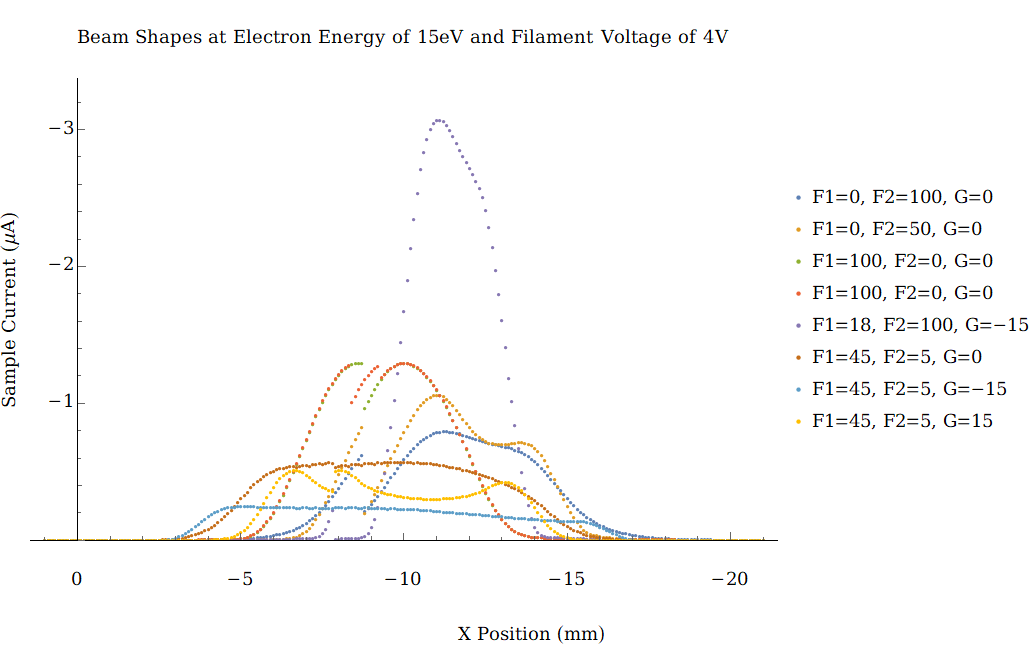
\includegraphics[width=0.85\linewidth]{../Work Term Replication/Plots/param sweep.png}
	\caption{Beam widths for varying $F1$, $F2$, and $G$ values at fixed $E_i=15$eV, $F=4$V and Ext$=100$V.}
    \label{fig:workterm}
\end{figure}

Standing out from all of the other configurations is one which has both the largest maximum current and the smallest beam width. The parameters 
used to create this beam are shown in table \ref{tab:optparam}. With this beam appearing to meet all of our requirements for inverse photoemission, 
we chose to characterize it further to see what improvements could be made.

\begin{table}[h!]
	\centering
	\begin{tabular}{ccccccc}
		\hline
		\multicolumn{1}{l|}{Paremeter} & Filament & Energy & Extraction & Grid & Focus 1 & Focus 2 \\ \hline
		\multicolumn{1}{l|}{Value (V)} & 4.0 & 15.0 & 100.0 & -15.0 & 18.0 & 100.0 \\ \hline
	\end{tabular}
	\caption{Gun parameters used to obtain the large, narrow beam shown in figure \ref{fig:workterm}}
	\label{tab:optparam}
\end{table}

\clearpage
\subsection{Characterizing the Optimized Beam}

The divergence angle of a beam can be used to determine the parallel component of a beam's momentum, making it a vital quantity to calculate if 
one wants to characterize an electron beam for inverse photoemission. To accomplish this, a longitudinal scan along the beams axis was conducted, 
measuring its width at varying working distances. Figure \ref{fig:long} shows the hyperbolic profile of the beam made up of individual beam width 
scans at set $y$ positions. 

\begin{figure}[h!]
    \centering
    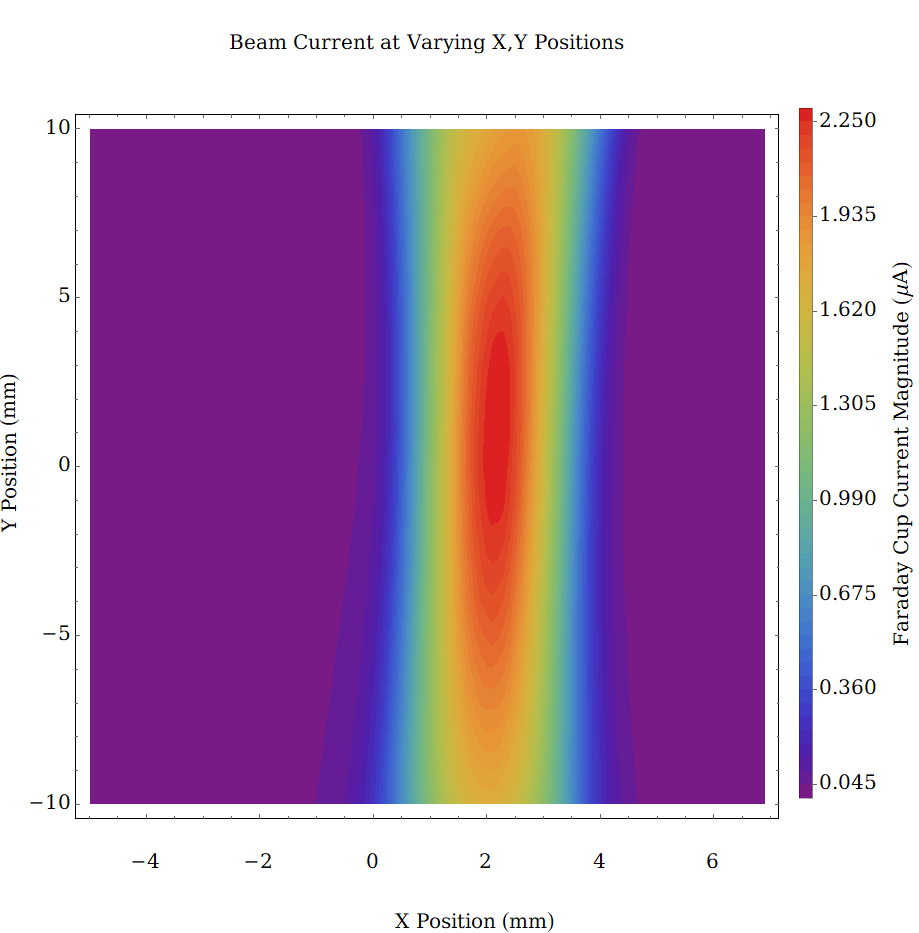
\includegraphics[width=0.85\linewidth]{../Beam Divergence/Plots/BeamwidthContour.png}
	\caption{Beam width as a function of distance along beam axis}
    \label{fig:long}
\end{figure}

A general gaussian of the form:

\begin{equation}
	I(x) = a \exp{\left(-\frac{(x-b^2)}{2c^2}\right)}
\end{equation}

was fitted to the current-position data. The full width at half maximum (FWHM) was used as the beam's width, and it is found using:

\begin{equation}
	\mathrm{FWHM} = 2\sqrt{2\ln2}c
\end{equation}

Figure \ref{fig:FWHM} shows how the FWHM changes along the beam's axis. 

\begin{figure}[h!]
    \centering
    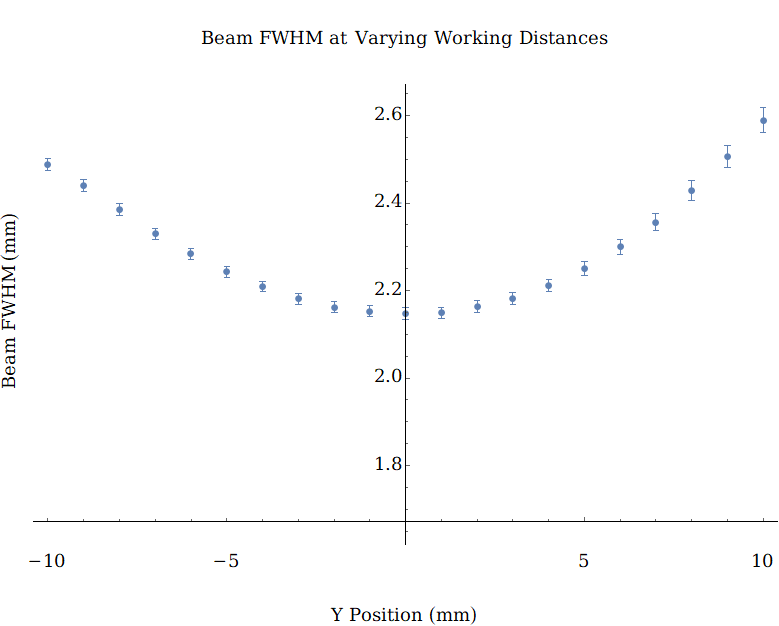
\includegraphics[width=0.85\linewidth]{../Beam Divergence/Plots/FWHM plot.png}
	\caption{FWHM as a function of distance along beam axis. Uncertainty was estimated using the standard deviation of fit parameters}
    \label{fig:FWHM}
\end{figure}

The divergence angle of a gaussian beam, $\Theta$, can be found using:

\begin{equation}
	\Theta = 2\arctan\left(\frac{D_f - D_i}{2\ell}\right)
\end{equation}

Where $D_f$ and $D_i$ are two separate beam diameters far from the beam's focus, and $\ell$ is the distance separating them. Using this the beam 
divergence angle was found to be $4.15\pm0.50^\circ$. 

As a final beam width scan, we can perform a raster in $x$ and $z$ to get a qualitative sense of the beams axial symmetry. The results of this 
are presented in figure \ref{fig:raster}.

\clearpage
\begin{figure}[h!]
    \centering
    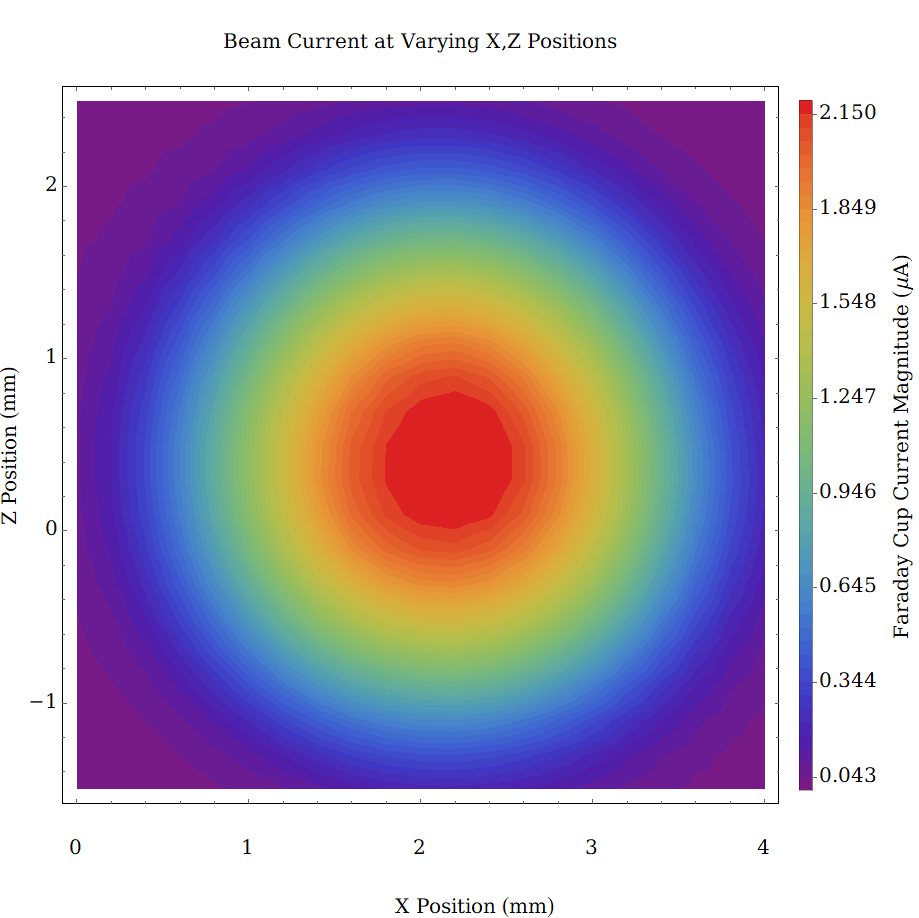
\includegraphics[width=0.85\linewidth]{../Beam Divergence/Plots/Raster plot.png}
	\caption{Raster scan of beam width in $x$ and $z$ directions, beam axis ($y$) is pointing into page.}
    \label{fig:raster}
\end{figure}

Finally, taking the derivative of equation \eqref{kpar} gives us the momentum resolution of the beam, $\Delta k_\parallel$, at an incidence angle $\theta$:

\begin{equation}
	\Delta k_\parallel = \frac{\sqrt{2m_e(E_k-\Delta)}}{\hbar}\cos\theta \Delta\theta
\end{equation}

Since the experiments were conducted at normal incidence we have $\theta=0$, and the angle broadening being given by $\Delta\theta = \frac{\Theta}{2}$.
From this we find the momentum spread of the beam to be\\$\Delta k_\parallel = (1.07\pm0.13)\times10^9\mathrm{m}^{-1}$.  

% \clearpage
\subsection{KRIPES Test on Cu(111) Single Crystal}

After finding a beam which met the criteria for inverse photoemission spectroscopy, and having previously characterized the system's photodetection
capabilities, we decided that as a final test we would attempt a k-resolved measurement of Cu(111). In inverse photoemission spectroscopy there 
are several samples which have been widely reported on in literature and serve as benchmarks spectrometer performance. One such example is the 
Cu(111) L-gap surface state, reported on by Budke et al. \cite{budke}, with expected results shown in figure \ref{fig:budke}. The state has a parabolic 
dispersion in $k_\parallel$, and appears as a peak roughly 0.25eV above the fermi energy. The L-gap state intensity grows sharply after an incidence angle 
of roughly $6^\circ$. 

\begin{figure}[h!]
	\centering
	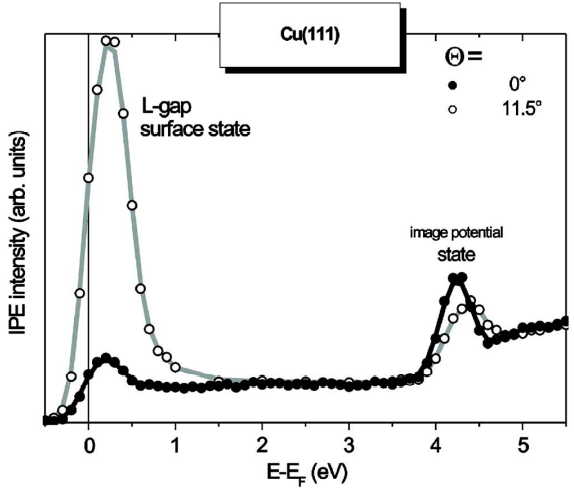
\includegraphics[width=0.45\linewidth, align=c]{../Assets/budke.png}
	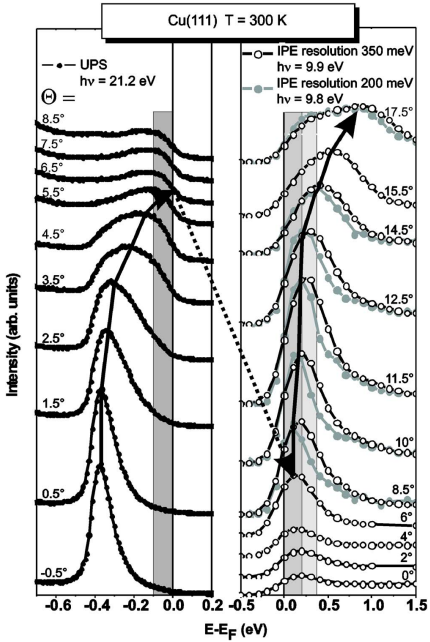
\includegraphics[width=0.45\linewidth, align=c]{../Assets/budke2.png}
	\caption{Left: K-resolved inverse photoemission spectra of Cu(111) at incidence angles of $0^\circ$ and $11.5^\circ$. Right:
	K-resolved measurements of L-gap state on Cu(111) (right subfigure) showing parabolic $k_\parallel$ dispersion\cite{budke}}
	\label{fig:budke}
\end{figure}

To replicate this we varied $E_i$ from 10eV to 20eV and recorded the resulting photon intensity. After a scan was completed, the incidence angle $\theta$
was varied using the rotational motor and another scan was performed. A selection of the spectra gathered is presented in figure \ref{fig:ipes}. 
Unfortunately no surface state was visible in the results, and an incident which ocurred later on left the sample in a state unfit for future trials. 

\clearpage
\begin{figure}[h!]
	\centering
	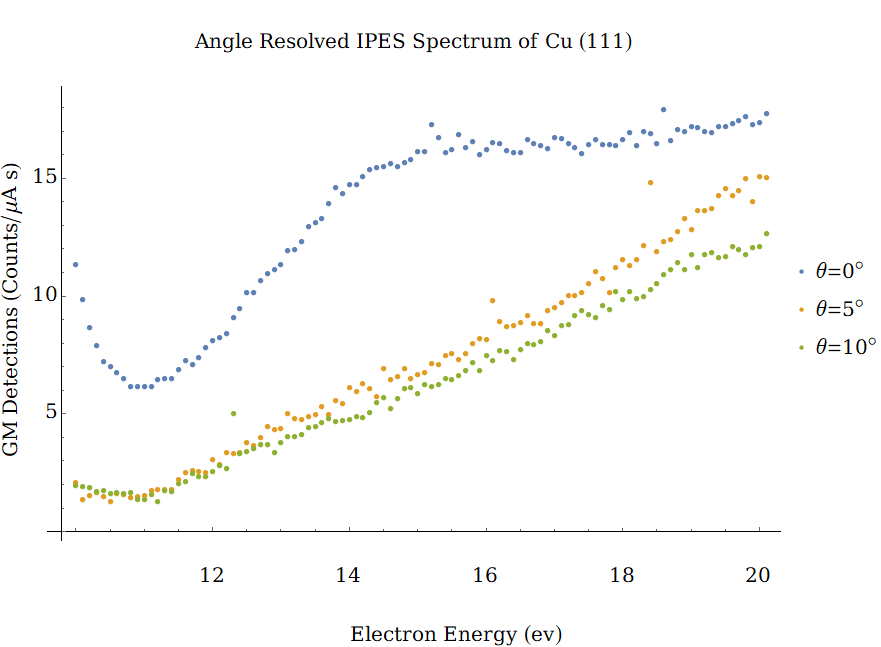
\includegraphics[width=0.85\linewidth]{../Cu 111 ARIPES/Plots/Better angle resolved.png}
	\caption{KRIPES of Cu(111) single crystal at incidence angles of 0$^\circ$, 5$^\circ$, and 10$^\circ$}
	\label{fig:ipes}
\end{figure}